% learn about REVTeX at https://journals.aps.org/revtex
% useful references:
%   https://cdn.journals.aps.org/files/revtex/summary4-1.pdf
%   ftp://ftp.dante.de/tex-archive/info/latex-refsheet/LaTeX_RefSheet.pdf
%   http://www-groups.mcs.st-andrews.ac.uk/~alanc/pub/c_tikzref/c_tikzref.pdf
\documentclass[
%draft,
aps,prd,
preprint,
onecolumn,
12pt,
amsmath, amssymb,
secnumarabic,
]{revtex4-1}

\usepackage[utf8]{inputenc}
\usepackage[english]{babel}
\usepackage{hyperref}
\usepackage[dvipsnames]{xcolor}
\usepackage{standalone}
\usepackage{multirow}
\usepackage{longtable}
\usepackage{graphicx}
\usepackage{tikz}
\usepackage{minted}
\usepackage{siunitx}
\usepackage[italicdiff]{physics}

\hypersetup{%
colorlinks=true,
linkcolor=RoyalBlue,
urlcolor=RoyalBlue,
citecolor=RoyalBlue,
}
\usetikzlibrary{decorations.markings}
\usetikzlibrary{calc}
\graphicspath{{../png/}}
\usemintedstyle{vs}
\definecolor{LightGray}{gray}{.9}
\setminted[python]{%
bgcolor=LightGray,
mathescape=true,
python3=true,
baselinestretch=1,
}

\newcommand{\comment}[1]{}
\newcommand{\python}[1]{\textcolor{BrickRed}{\texttt{#1}}}

\begin{document}

\title{Gravispy: gravitational simulations in open source software}
\homepage{https://github.com/cjayross/gravispy}
\author{Spence Norwood}
\author{Kellen O'Keefe}
\author{Calvin Ross}
\affiliation{University of Texas at Dallas, Physics Department}
\begin{abstract}
Gravispy is designed to demonstrate the effects of gravitational lensing on light through the calculation of a massive object’s effect on local spacetime and by using the obtained result to visualize the phenomenon in a three dimensional representation. Through the usage of the Gauss-Kronrod quadrature formula and the Brent-Dekker method, numerical solutions are found to the curvature magnitude of light in the vicinity of a black hole, and are used to create a mapping to the light of an unperturbed state. The mapping is used to transform an image of unwarped spacetime to an image of the same environment but near a black hole. This resultant image is projected onto a sphere using OpenGL to provide a panoramic view of the environment. The results of this project have been generally successful. Gravitational lensing has been correctly modeled, with the exception of a small shearing of the image, and the lensing effect is viewable in a three dimensional model. Initial goals were to make the simulation dynamic, but currently only a static simulation is supported. Future improvements to this project could be made by implementing this functionality, and by increasing the accuracy of the simulation by modeling the effect of blueshift and the creation of hidden images.
\end{abstract}
\maketitle

\section{Introduction\label{sec:intro}}
\documentclass{standalone}

\begin{document}


\end{document}


\section{Motivation\label{sec:motive}}
\documentclass{standalone}

\begin{document}


\end{document}


\section{Methods\label{sec:method}}
\documentclass{standalone}

\begin{document}

\begin{figure*}
  \caption{\label{fig:imgbuild}
    Illustration marking intermediary steps during the image forming process.
    The new image is first created that defaults to black.
    During execution, the \emph{apply\_lens} algorithm iterates through each pixel of the newly generated image and uses the passed lensing map to determine which pixel from the input should be placed at that location.}
  \begin{tikzpicture}[>=stealth,line width=3pt]
    \tikzset{every node/.style={inner sep=0pt}}
    \def\voffset{3.75cm}
    \def\hoffset{5cm}
    \node (in) at (-\hoffset,0pt)
      {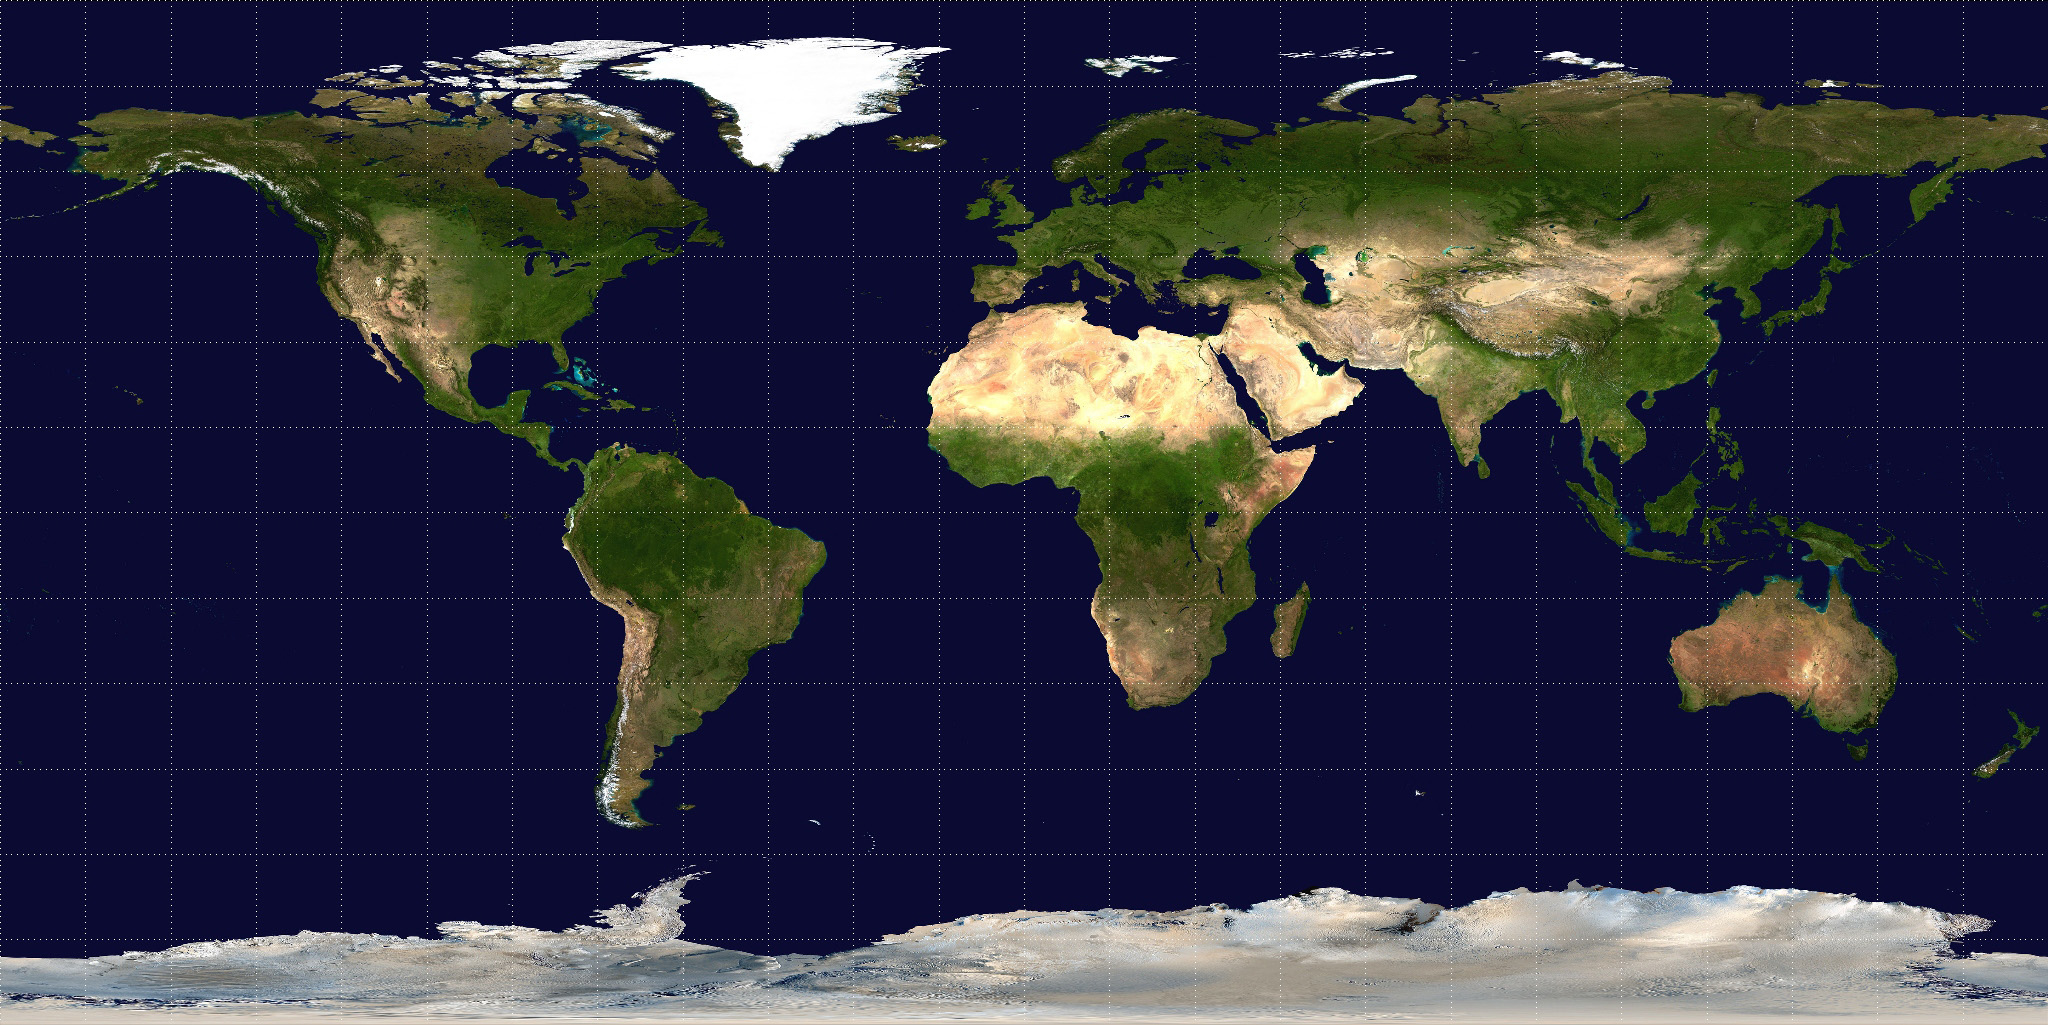
\includegraphics[width=.4\textwidth]{earth}};
    \node (out1) at (\hoffset,\voffset)
      {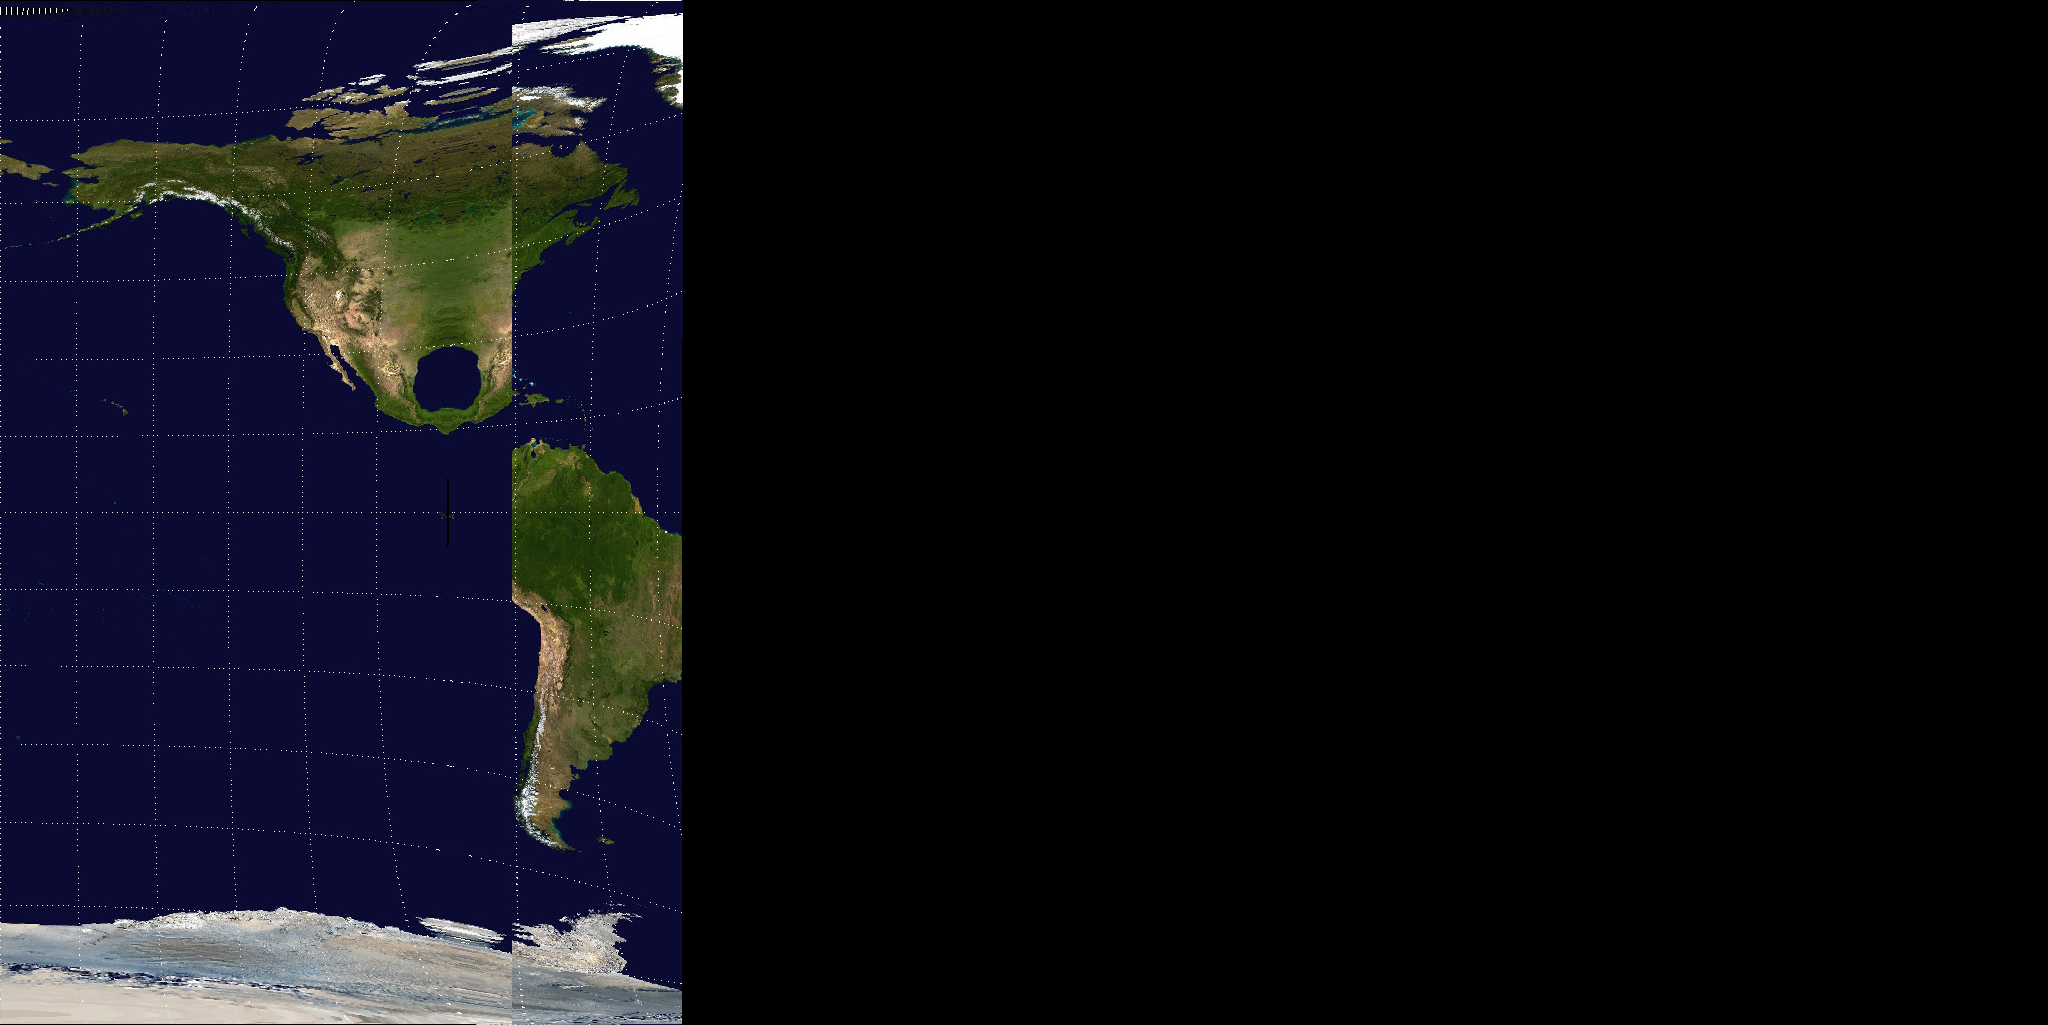
\includegraphics[width=.35\textwidth]{output_onethird}};
    \node (out2) at (\hoffset,0pt)
      {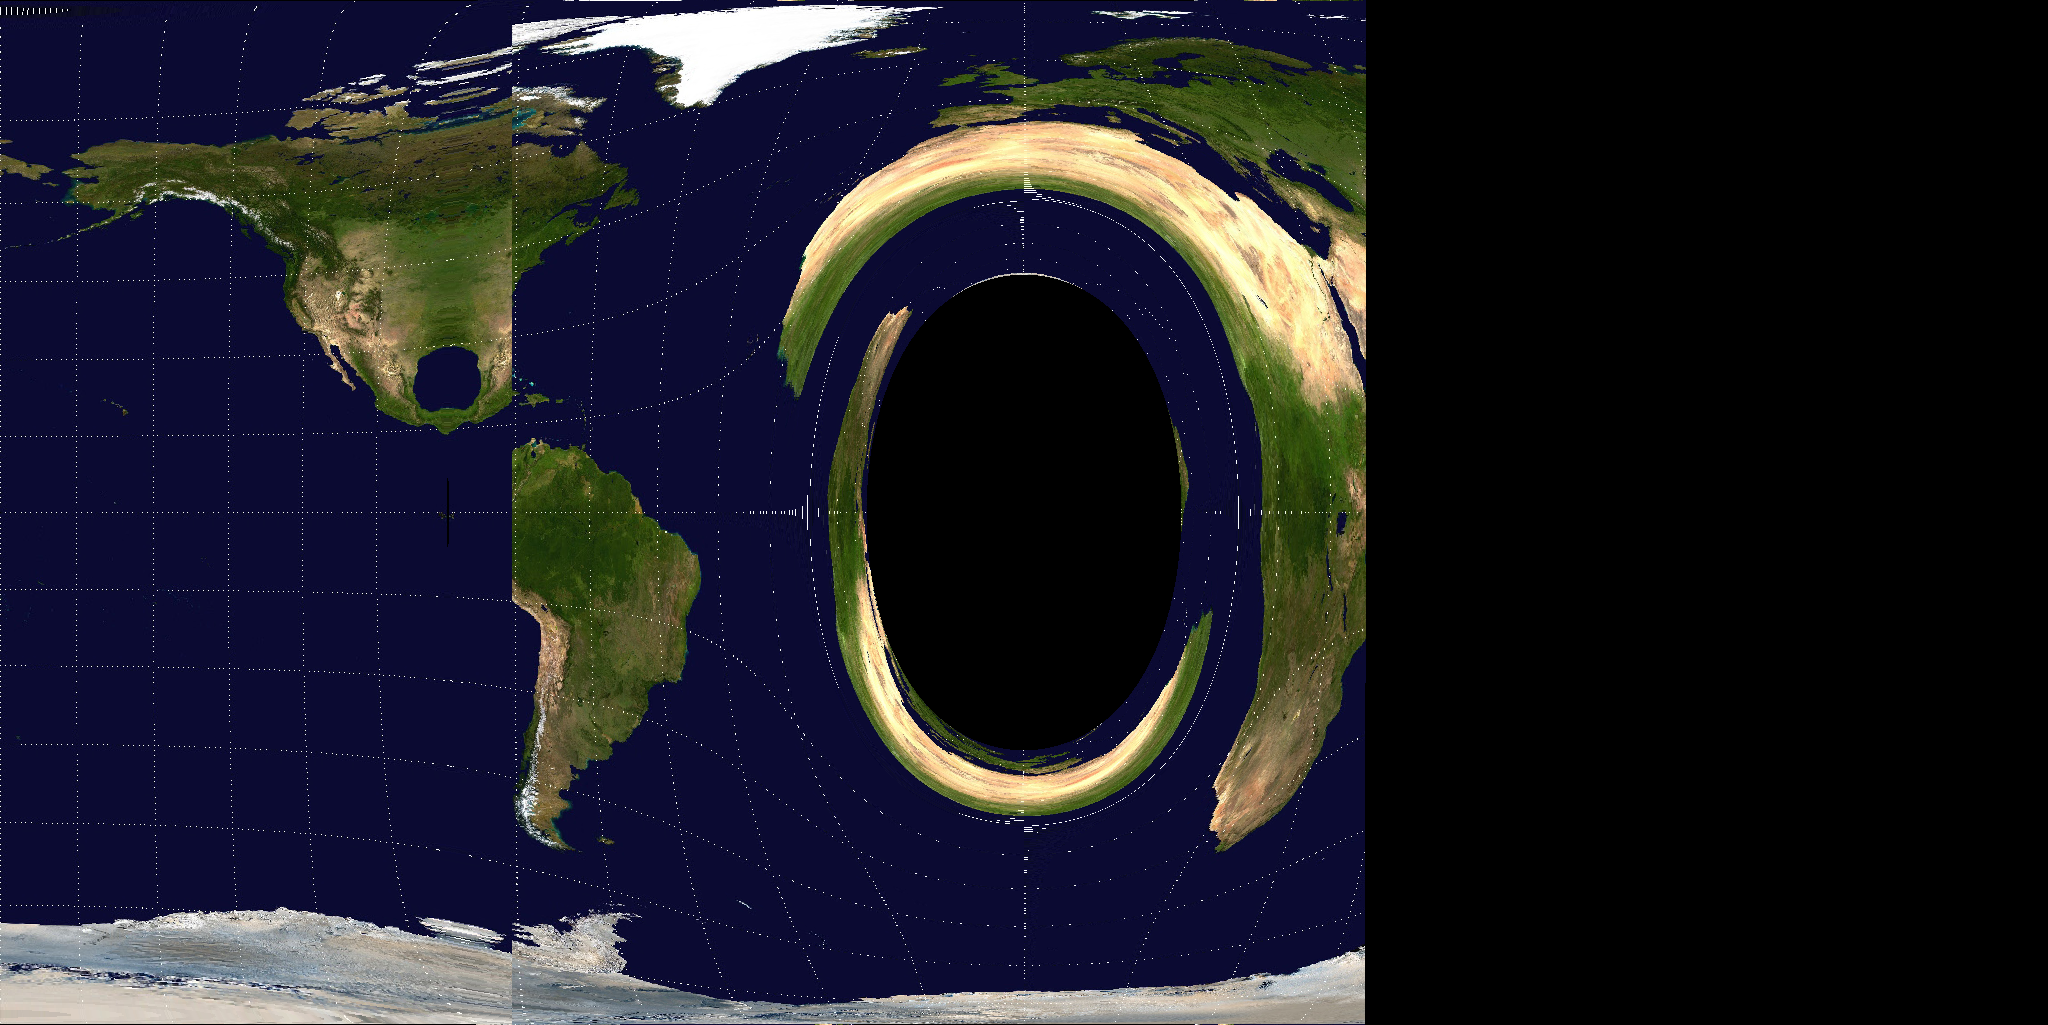
\includegraphics[width=.35\textwidth]{output_twothird}};
    \node (out3) at (\hoffset,-\voffset)
      {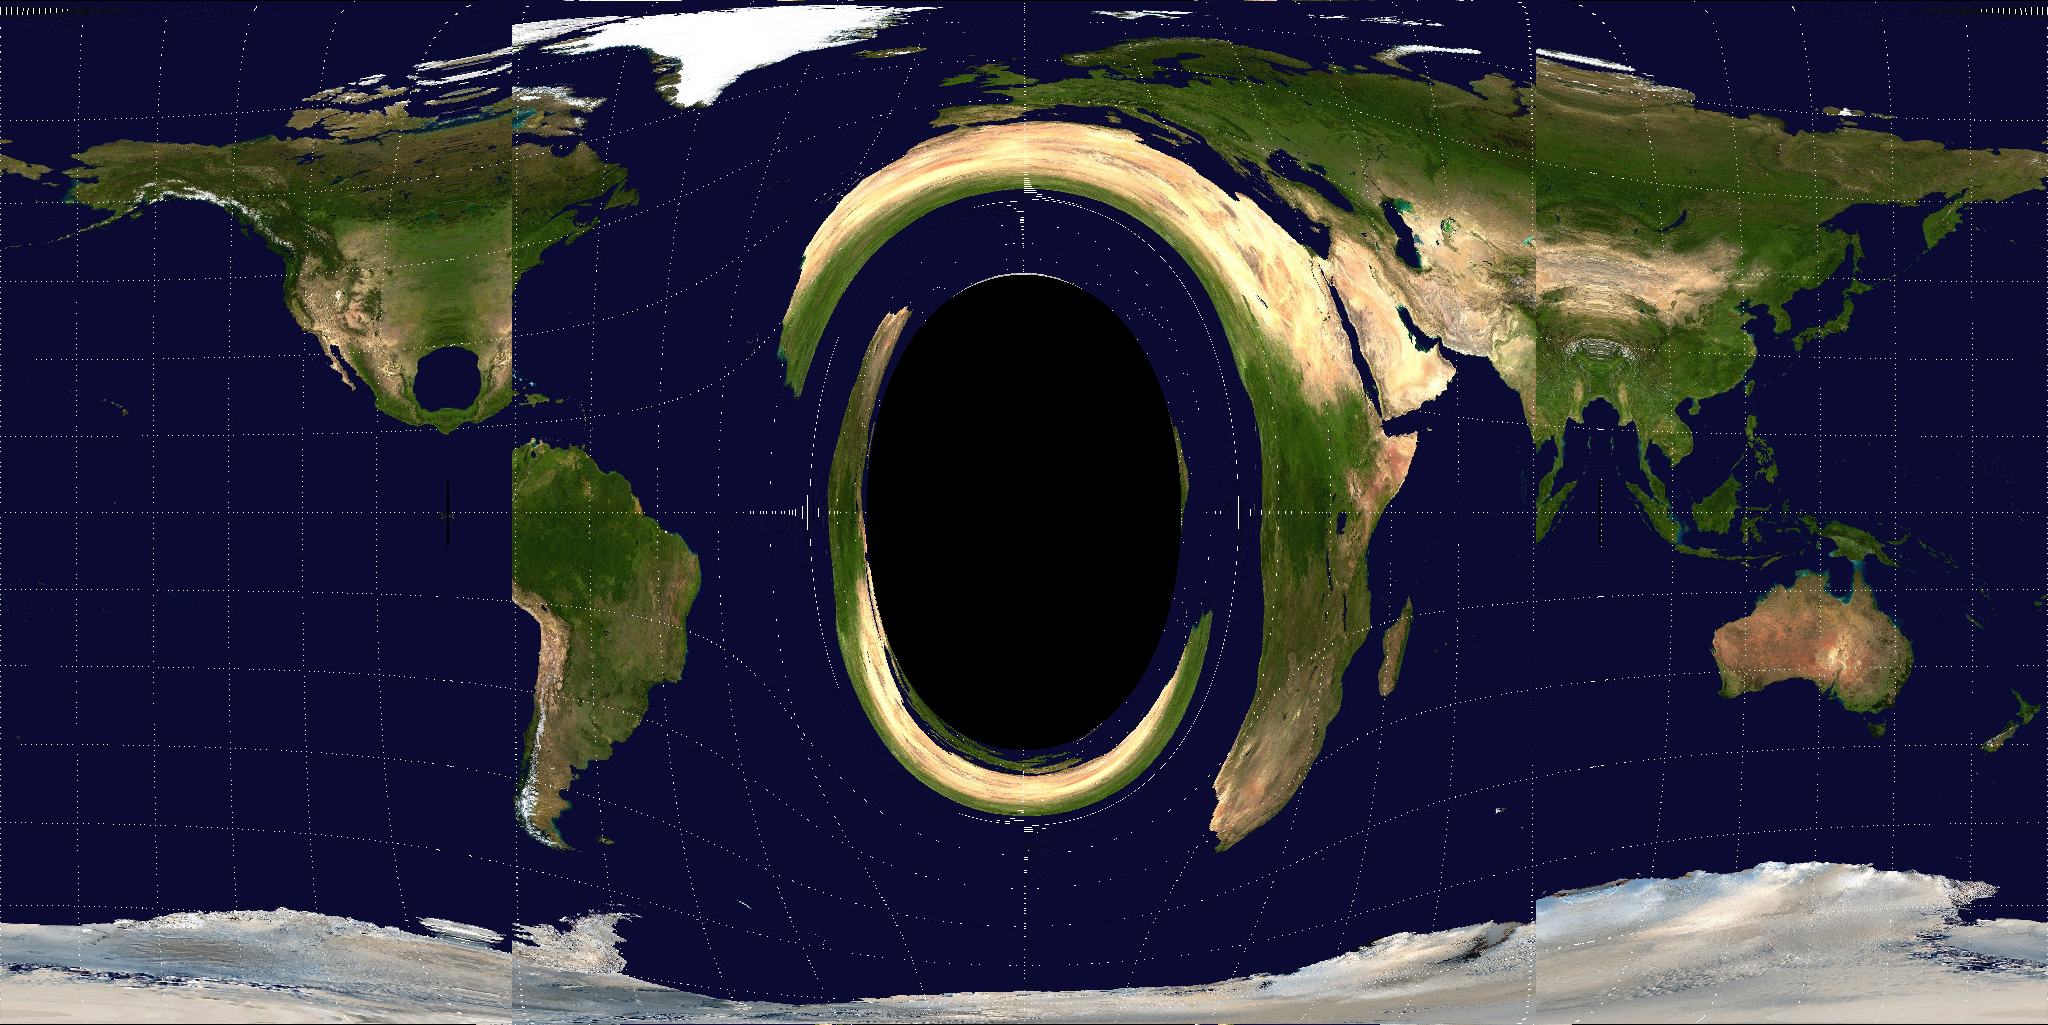
\includegraphics[width=.35\textwidth]{output_full}};
    \draw[->,shorten <=5mm,shorten >=5mm] (in) -- (out2);
    \draw[->] (out1) -- (out2);
    \draw[->] (out2) -- (out3);
  \end{tikzpicture}
\end{figure*}

\end{document}


\section{Results\label{sec:results}}
\documentclass{standalone}

\begin{document}
\begin{figure*}
  \caption{\label{fig:earthsample}
    Sample image used to test the application of a generated lensing map.
  }
  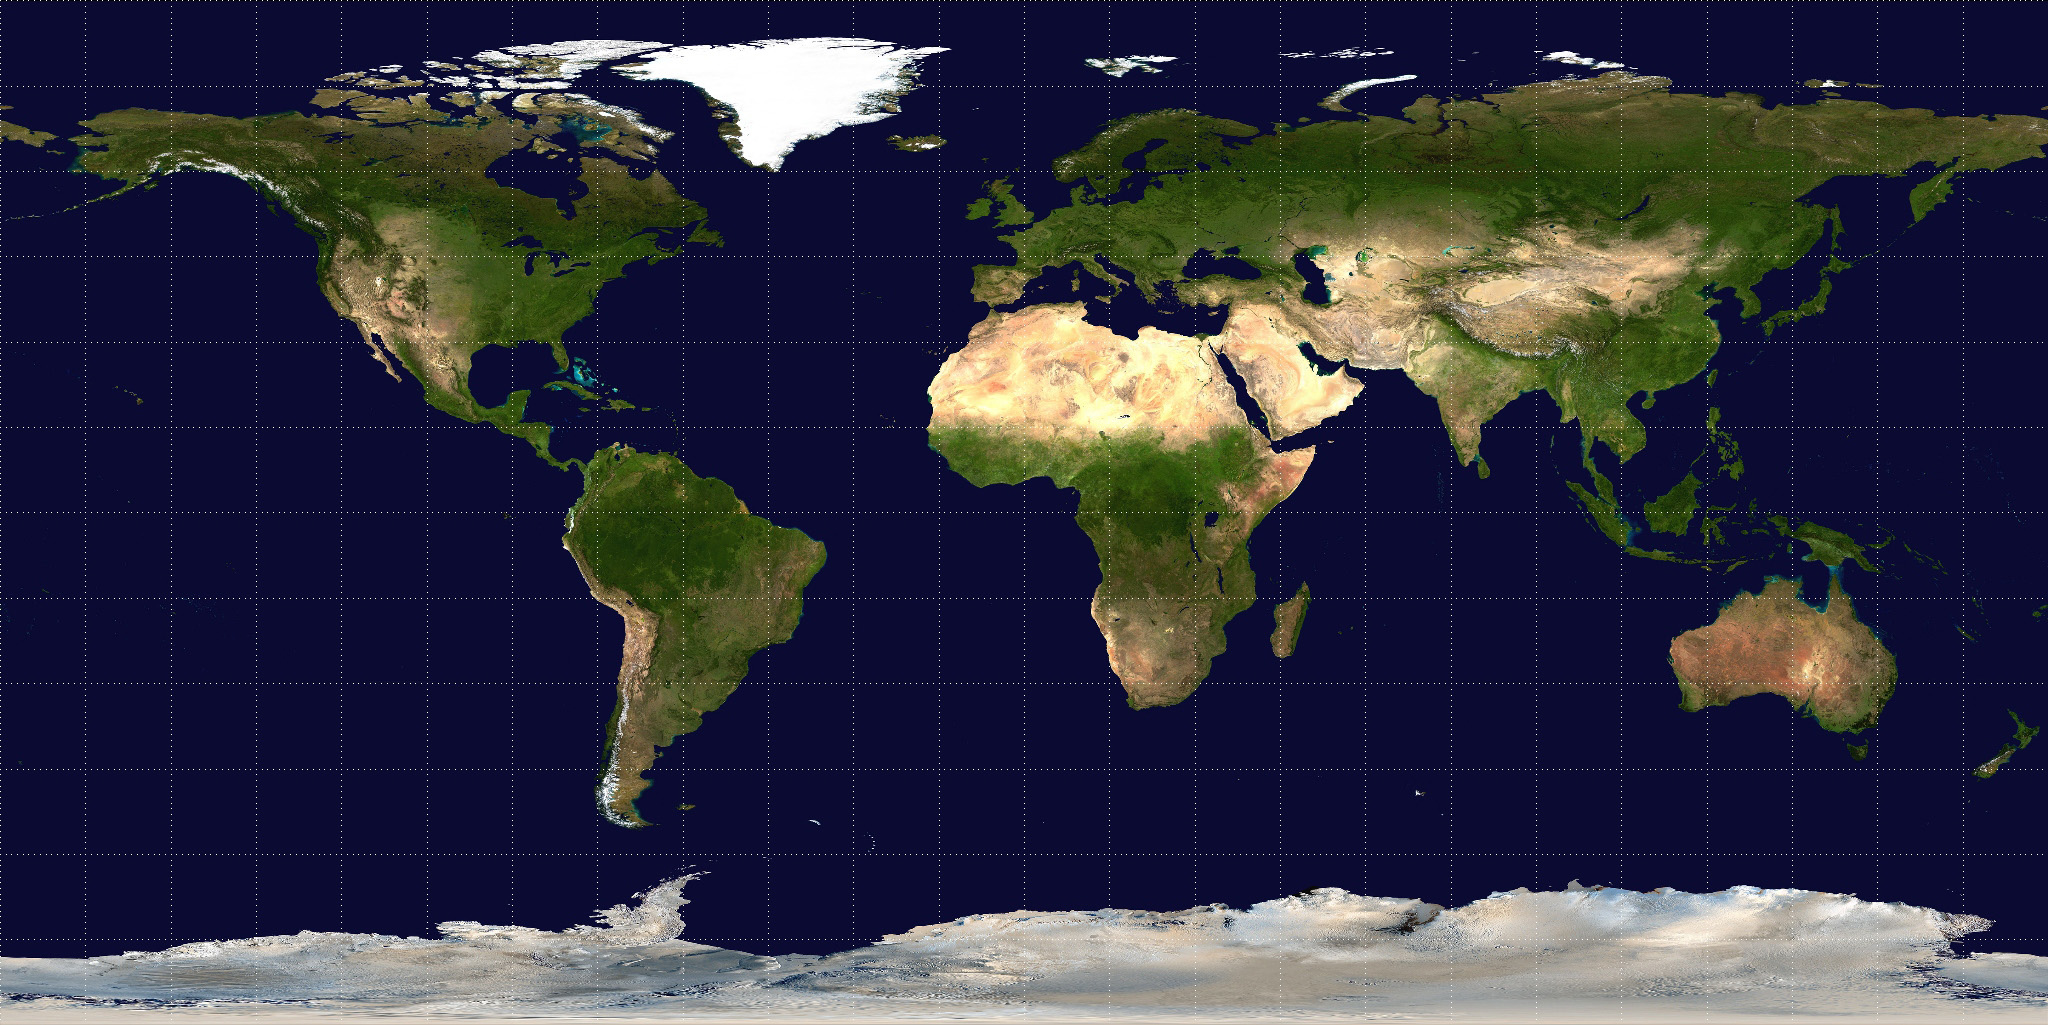
\includegraphics[width=\textwidth]{earth}
\end{figure*}

\begin{figure*}
  \caption{\label{fig:example1}
    Final result of applying the explicit Schwarzschild lensing map on the sample image shown in Fig.(\ref{fig:earthsample}) using a Schwarzschild space-time defined by $M=\SI{1}{\kilo\meter}$ and $R_O=\SI{10}{\kilo\meter}$.
    In this example, one can easily see the problematic image tearing at the $\pi/2$ and $-\pi/2$ meridians.
  }
  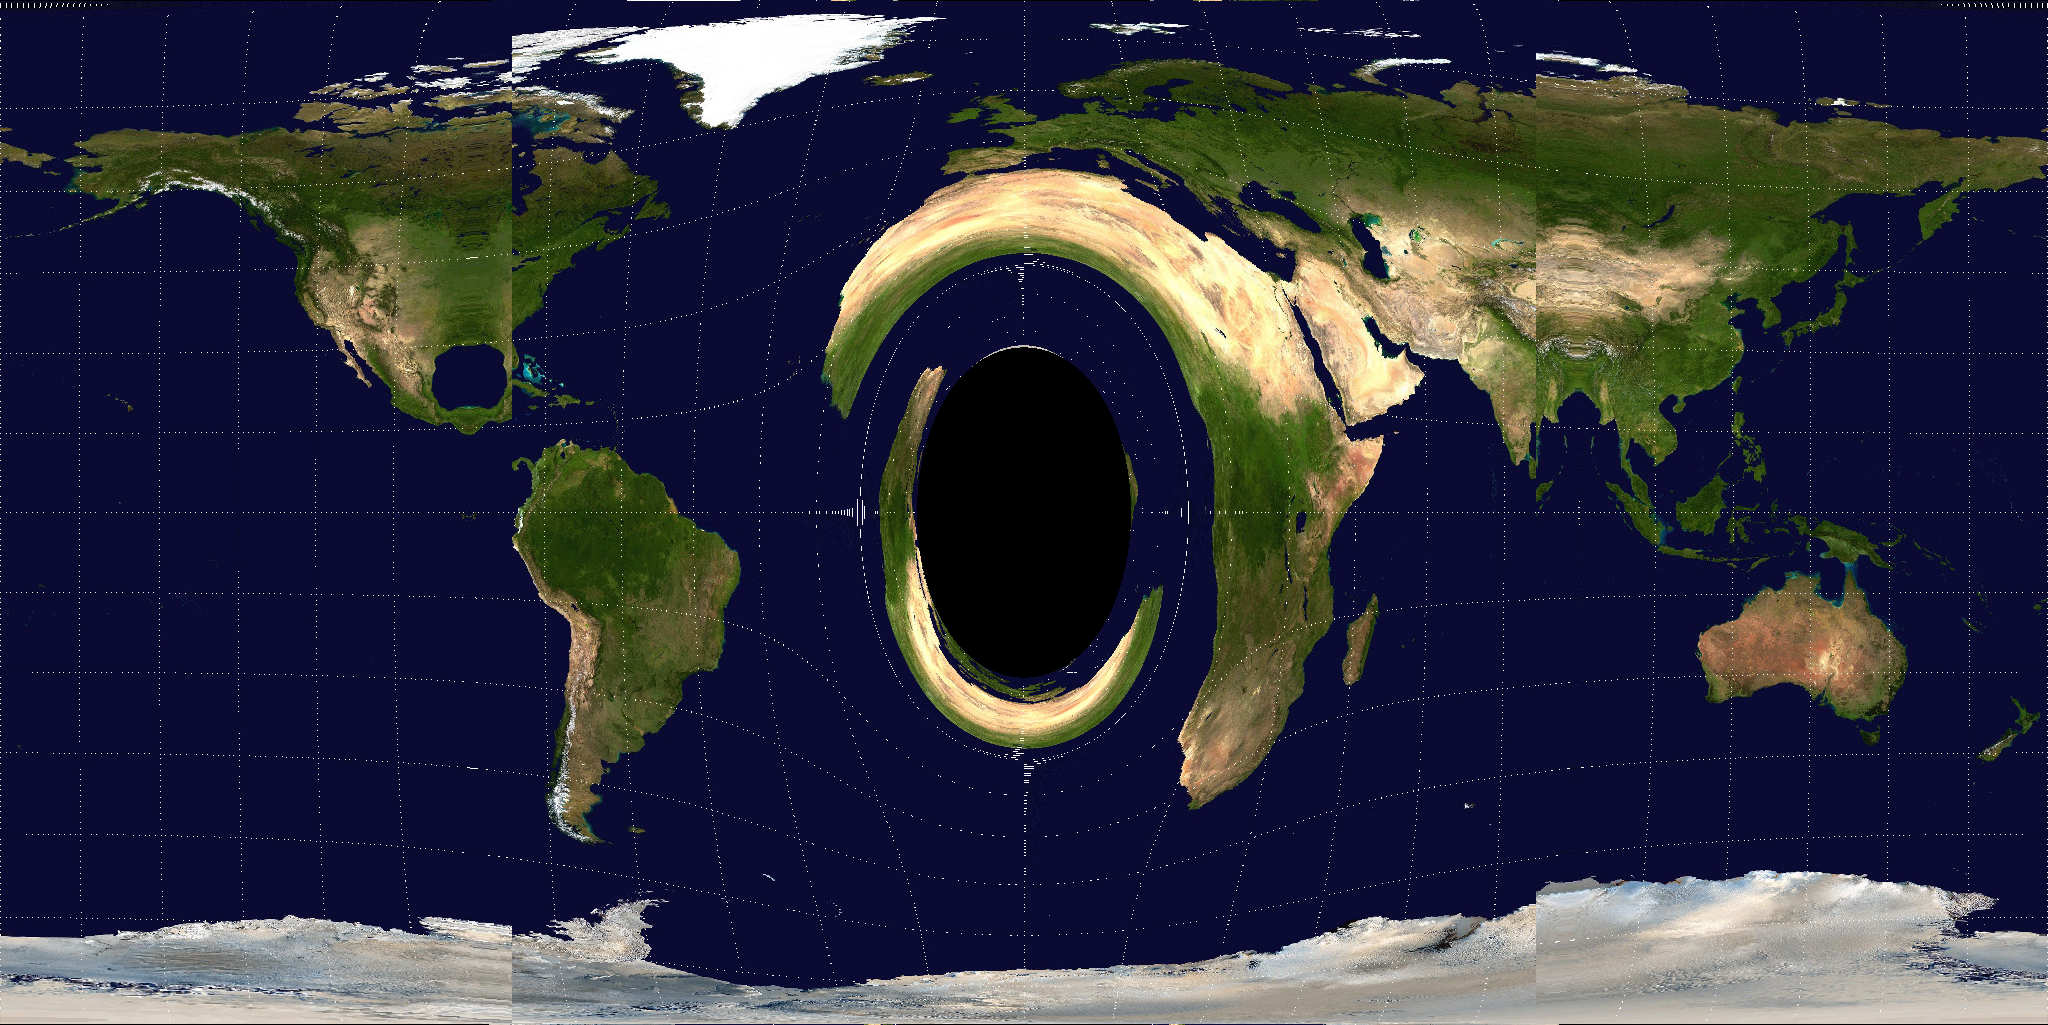
\includegraphics[width=\textwidth]{example_lens1}
\end{figure*}

\begin{figure*}
  \caption{\label{fig:example2}
    Second example of a generated Schwarzschild lensing map using the same space-time as in Fig.(\ref{fig:example1}) but at a radius of $R_O=\SI{2.5}{\kilo\meter}$, which is significantly closer to the event horizon.
    The accuracy of this result hasn't yet been scrutinized, however the overall converging of the observer's sky to the point at $\phi=0$ is to be expected.
  }
  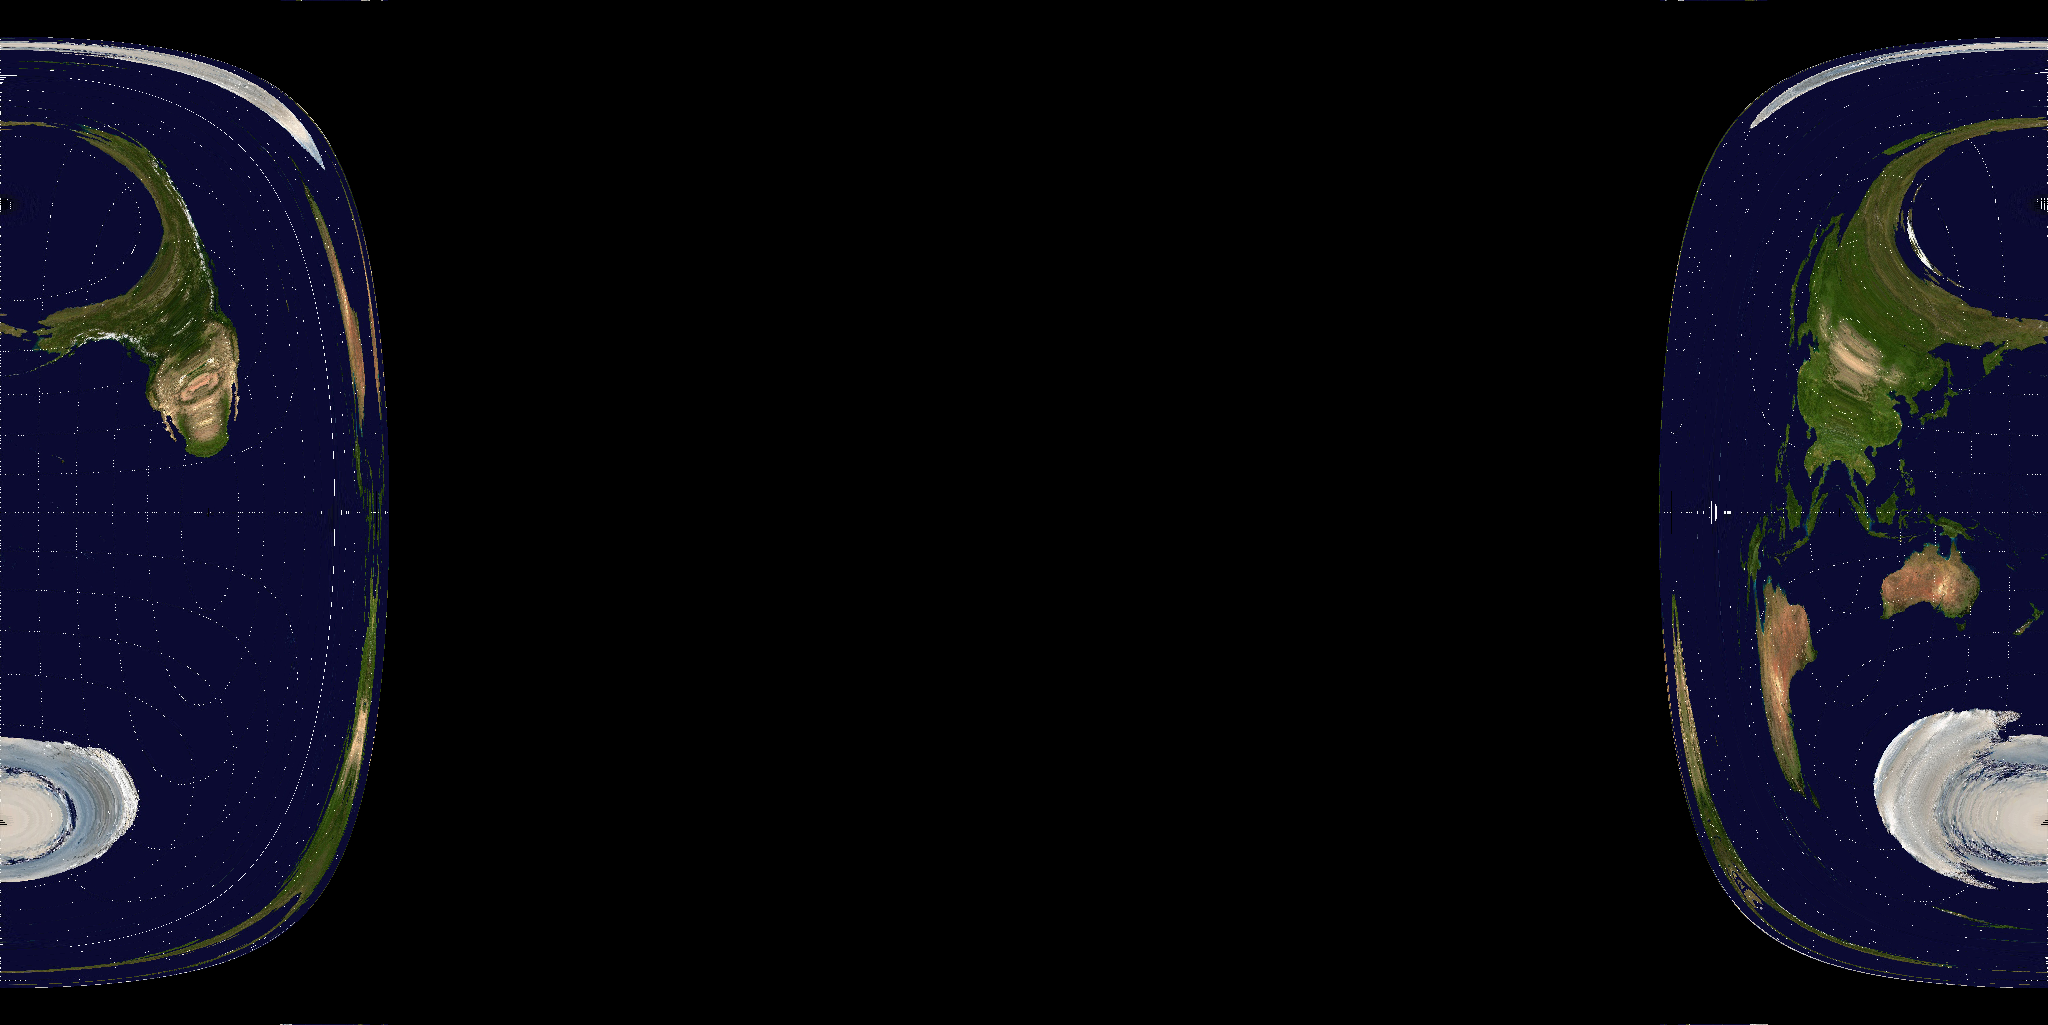
\includegraphics[width=\textwidth]{example_lens2}
\end{figure*}

\begin{figure*}
  \caption{\label{fig:lenscomparison}
    Comparison between the three levels of approximation in the Schwarzschild lensing equation.
    The first graph indicates the differences near the singularity, while the latter shows that the amount of error decreases significantly as the radius of the observer increases.
  }
  \begin{tabular}{c}
    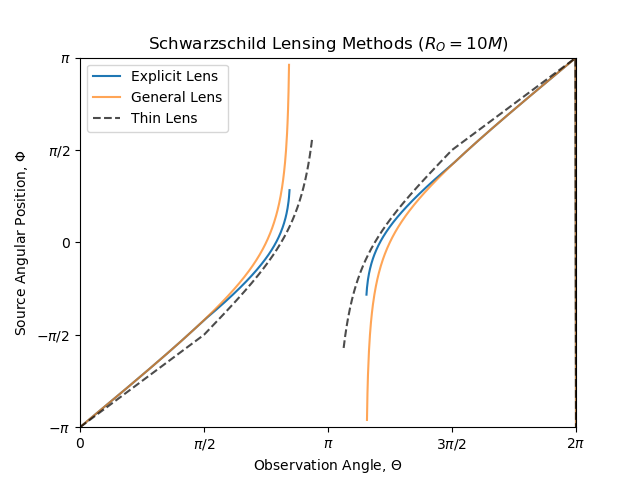
\includegraphics[width=.75\textwidth]{sc_lensing_near}\\
    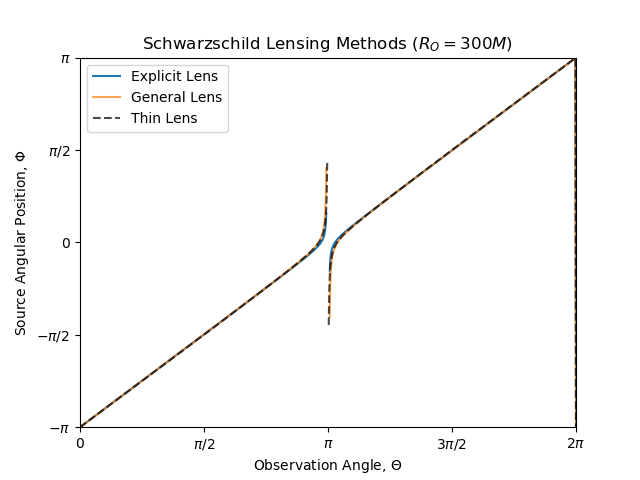
\includegraphics[width=.75\textwidth]{sc_lensing_far}
  \end{tabular}
\end{figure*}

\end{document}


\section{Discussion and Conclusion}
\documentclass{standalone}

\begin{document}


\end{document}


\nocite{*}
\bibliography{report}

\end{document}
